\chapter{Geschlossene Strings, Level-Matching und Dualität}

\lectureoverview{Ein geschlossener String trägt unabhängige Wellen in seinen beiden intrinsischen Richtungen. Bei der Quantisierung scheint sich dadurch zunächst das Photon des offenen Strings zu verdoppeln, doch die Invarianz gegenüber einer Verschiebung des Ursprungs der Stringkoordinate schließt die einseitigen Zustände aus. Die erste verbleibende Stufe enthält ein masseloses Spin-2-Teilchen. Die Idee, Beschreibungen zu ändern, führt dann zu einer weiter gefassten Frage: Was bedeutet es bei veränderlichen Kopplungen, dass irgendein Objekt fundamental ist?}

\section{Ein Generator in Reserve}

Rufen wir uns, bevor wir einen geschlossenen String zeichnen, eine Tatsache aus der kanonischen Mechanik in Erinnerung. Es sei
\begin{equation}
  L=L(q_i,\dot q_i),
\end{equation}
und der zu \(q_i\) kanonisch konjugierte Impuls sei definiert durch
\begin{equation}
  p_i=\frac{\partial L}{\partial\dot q_i}.
\end{equation}
Eine infinitesimale kontinuierliche Transformation lässt sich schreiben als
\begin{equation}
  \delta q_i=\epsilon f_i(q),
  \label{eq:l04-infinitesimal-transformation}
\end{equation}
wobei \(\epsilon\) ein kleiner Parameter ist. Ist diese Transformation eine Symmetrie, so liefert der Satz von Noether eine erhaltene Ladung. Teilt man die Koordinatenverschiebung durch den gemeinsamen Parameter, erhält man den Generator
\begin{equation}
  Q=\sum_i p_i f_i(q)
   =\frac{1}{\epsilon}\sum_i p_i\,\delta q_i.
  \label{eq:l04-noether-charge}
\end{equation}
In der Quantenmechanik ist \(Q\) der Operator, der die entsprechende kleine Transformation erzeugt.

Eine Rotation in der \(xy\)-Ebene ist das vertraute Beispiel. Bei einer bestimmten Wahl der Orientierung gilt
\begin{equation}
  \delta x=\epsilon y,
  \qquad
  \delta y=-\epsilon x,
\end{equation}
und \eqref{eq:l04-noether-charge} wird bis auf dieselbe Vorzeichenwahl zum Drehimpuls. Auf das konkrete Beispiel kommt es nicht an. Entscheidend ist das Muster: Der mit der infinitesimalen Verschiebung kontrahierte Impuls ergibt den Generator.

\begin{figure}[H]
  \centering
  \includegraphics[width=0.76\textwidth]{lecture_04_figure_01.png}
  \caption{Der kanonische Impuls und der Noether-Generator, die für die spätere Verschiebung der Koordinate des geschlossenen Strings aufbewahrt werden.}
  \lectureframe{00:05:00}
  \label{fig:l04-noether-board}
\end{figure}

Bald begegnen wir einer Symmetrie, deren Koordinate kein Punkt im gewöhnlichen Raum ist, sondern die Bezeichnung von Punkten entlang eines Strings. Gleichung \eqref{eq:l04-noether-charge} wird zu diesem Zweck bereitgestellt.

\section{Eine Koordinate um eine Schleife}

Ein geschlossener String hat keine Endpunkte. Wählen wir einen Parameter
\begin{equation}
  0\leq \sigma<2\pi
\end{equation}
und markieren wir vorerst einen Punkt als \(\sigma=0\). Der gegenüberliegende Punkt ist \(\sigma=\pi\); eine Vierteldrehung und eine Dreivierteldrehung entsprechen \(\pi/2\) und \(3\pi/2\). Die Markierung legt eine Koordinatenkonvention fest, zunächst aber kein physikalisches Merkmal.

\begin{figure}[H]
  \centering
  \begin{minipage}[t]{0.58\textwidth}
    \centering
    \includegraphics[width=\textwidth]{lecture_04_figure_02.png}
    \par\smallskip\footnotesize (a) Die markierte Schleife an der Tafel.
  \end{minipage}\hfill
  \begin{minipage}[t]{0.37\textwidth}
    \centering
    \begin{adjustbox}{max width=\linewidth}
    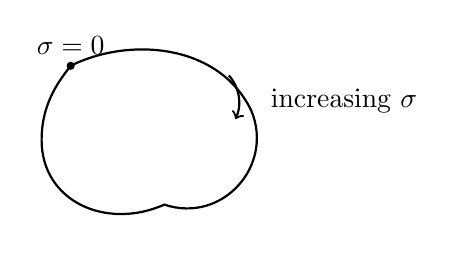
\begin{tikzpicture}[scale=0.82]
      \draw[thick]
        (0.1,1.1)
        .. controls (1.0,1.55) and (2.4,1.45) .. (2.9,0.4)
        .. controls (3.25,-0.45) and (2.45,-1.35) .. (1.55,-1.05)
        .. controls (0.65,-1.45) and (-0.35,-1.0) .. (-0.35,-0.05)
        .. controls (-0.35,0.55) and (-0.05,0.9) .. (0.1,1.1);
      \fill (0.1,1.1) circle (1.8pt);
      \node[above] at (0.1,1.12) {\(\sigma=0\)};
      \draw[->,thick] (2.55,0.95) arc[start angle=42,end angle=-25,radius=0.62];
      \node[right] at (3.05,0.55) {increasing \(\sigma\)};
    \end{tikzpicture}
    \end{adjustbox}
    \par\smallskip\footnotesize (b) Die intrinsische Orientierung.
  \end{minipage}
  \caption{Ein Punkt wird markiert, um den Ursprung festzulegen, und ein Pfeil gibt die Richtung an, in der \(\sigma\) zunimmt.}
  \lectureframe{00:06:48}
  \label{fig:l04-closed-string-origin}
\end{figure}

Der Pfeil entlang der Schleife gibt eine \emph{intrinsische} Orientierung an. Sie darf nicht mit einer Bewegung im Uhrzeigersinn oder gegen den Uhrzeigersinn in der \(xy\)-Ebene verwechselt werden. Man stelle sich vor, ein markiertes Gummiband werde von der Tafel abgehoben, umgedreht und wieder abgelegt. Sein scheinbarer Umlaufsinn kehrt sich um, die Reihenfolge seiner intrinsischen Markierungen bleibt jedoch gleich. Zunehmendes \(\sigma\) bleibt zunehmendes \(\sigma\).

Diese Unterscheidung bestimmt, wie wir von rechts- und linkslaufenden Wellen sprechen. In diesem Kapitel bezeichnet eine rechtslaufende Störung eine Störung, die sich in Richtung zunehmenden \(\sigma\) bewegt; eine linkslaufende Störung bewegt sich in Richtung abnehmenden \(\sigma\). Keine der beiden Bezeichnungen sagt aus, in welche Richtung sich die Störung im Raum scheinbar bewegt.

Die Orientierung spielte im ursprünglichen hadronischen Stringbild eine konkrete Rolle. Beim Aufbrechen eines orientierten Flussrohrs entsteht an dem einen Ende ein Quark und am anderen ein Antiquark; der intrinsische Pfeil unterscheidet die beiden Enden. Man kann auch unorientierte Stringtheorien konstruieren, doch für die vorliegende Diskussion behalten wir den Pfeil und die beiden Richtungen entlang des Strings bei.

\section{Periodizität und laufende Wellen}

Seien \(X(\sigma,\tau)\) und \(Y(\sigma,\tau)\) zwei transversale Koordinaten des Strings, wobei \(\tau\) die Zeit bezeichnet. Zusätzliche transversale Koordinaten werden, falls vorhanden, genau gleich behandelt. Da \(\sigma=0\) und \(\sigma=2\pi\) denselben Punkt bezeichnen, gilt
\begin{equation}
  X(\sigma+2\pi,\tau)=X(\sigma,\tau),
  \qquad
  Y(\sigma+2\pi,\tau)=Y(\sigma,\tau).
  \label{eq:l04-periodicity}
\end{equation}

\begin{figure}[H]
  \centering
  \includegraphics[width=0.76\textwidth]{lecture_04_figure_03.png}
  \caption{Periodische Randbedingungen für die beiden transversalen Koordinaten.}
  \lectureframe{00:12:40}
  \label{fig:l04-periodicity-board}
\end{figure}

Eine lokalisierte Auslenkung kann daher unbegrenzt umlaufen. Erreicht sie \(2\pi\), erscheint sie einfach wieder bei \(0\). Das unterscheidet sich von einem offenen String, bei dem eine laufende Welle einen Endpunkt erreicht und reflektiert wird: Aus einer links laufenden wird eine rechts laufende Welle und umgekehrt. Beim offenen String sind stehende Wellen naheliegend, während ein geschlossener String zwei unabhängig laufende Wellenfamilien zulässt.

\subsection{Komplexe Fourier-Moden}

Eine zweckmäßige Basis für eine periodische Funktion ist
\begin{equation}
  e^{in\sigma}=\cos(n\sigma)+i\sin(n\sigma),
  \qquad n\in\mathbb Z.
\end{equation}
Die Ganzzahligkeit ist durch die Periodizität vorgegeben:
\(e^{in(\sigma+2\pi)}=e^{in\sigma}\). Ersetzt man \(n\) beispielsweise durch eine Halbzahl, ändert sich die Funktion nach einem Umlauf.

Lassen wir die Zeitabhängigkeit vorübergehend weg, so lautet die Entwicklung an der Tafel
\begin{align}
  X(\sigma)
  &=
  X_0+
  \sum_{n>0}X_n e^{in\sigma}
  +\sum_{n>0}X_{-n}e^{-in\sigma},
  \label{eq:l04-fourier-x}\\
  Y(\sigma)
  &=
  Y_0+
  \sum_{n>0}Y_n e^{in\sigma}
  +\sum_{n>0}Y_{-n}e^{-in\sigma}.
  \label{eq:l04-fourier-y}
\end{align}
Für reelle \(X\) und \(Y\) sind die Koeffizienten mit negativem Index auf klassischer Ebene die komplex konjugierten der Koeffizienten mit positivem Index. Die Nullmoden \(X_0\) und \(Y_0\) geben die Lage des Schwerpunkts an; sie sind Positionen und keine inneren Schwingungen.

\begin{figure}[H]
  \centering
  \includegraphics[width=0.82\textwidth]{lecture_04_figure_04.png}
  \caption{Die Anteile mit positivem und negativem Index der periodischen Fourier-Entwicklung, gefolgt von der Nullmode.}
  \lectureframe{00:20:00}
  \label{fig:l04-fourier-board}
\end{figure}

\begin{classroomqa}
\audiencequestion{Wo ist die Zeitkoordinate, wenn dies laufende Wellen sind?\lecturetimestamp{00:19:05}}
\lecturerresponse{In der Tafelnotation wurde sie lediglich unterdrückt. Die Phase einer laufenden Lösung hängt sowohl von \(\sigma\) als auch von \(\tau\) ab. Bei der unten verwendeten Konvention hat eine Familie die Form \(e^{-in(\tau-\sigma)}\), die andere die Form \(e^{-in(\tau+\sigma)}\).}
\end{classroomqa}

Für die Ausbreitung ist also die vollständige Phase maßgeblich, nicht allein das Vorzeichen von \(n\) in einem rein räumlichen Fourier-Faktor. Wir können schreiben
\begin{equation}
  X(\sigma,\tau)=X_R(\tau-\sigma)+X_L(\tau+\sigma),
  \label{eq:l04-chiral-solution}
\end{equation}
und entsprechend für \(Y\). Welche Familie als \(R\) und welche als \(L\) bezeichnet wird, ist Konvention; invariant ist die Tatsache, dass es entlang des \(\sigma\)-Kreises zwei entgegengesetzte Richtungen gibt.\editorialnote{\(e^{in\sigma}\) legt für sich allein zu einem einzelnen Zeitpunkt noch keine laufende Welle fest. Die Ausbreitung ist erst bestimmt, wenn die Zeitphase angegeben ist.}

\section{Energie in den beiden Richtungen}

Die lokale Dynamik ist dieselbe wie beim offenen String. In der hier verwendeten vereinfachten Normierung gilt
\begin{equation}
  L\propto
  \int_0^{2\pi}d\sigma\,
  \left[
    \dot X^2-X'^2+\dot Y^2-Y'^2
  \right],
  \label{eq:l04-string-lagrangian}
\end{equation}
wobei ein Punkt \(\partial_\tau\) und ein Strich \(\partial_\sigma\) bezeichnet. In der Energie steht zwischen kinetischem und elastischem Term ein Pluszeichen:
\begin{equation}
  E\propto
  \int_0^{2\pi}d\sigma\,
  \left[
    \dot X^2+X'^2+\dot Y^2+Y'^2
  \right].
  \label{eq:l04-string-energy}
\end{equation}
Für jede der beiden transversalen Koordinaten gilt
\begin{equation}
  \dot X^2+X'^2
  =
  \frac12(\dot X+X')^2+
  \frac12(\dot X-X')^2.
  \label{eq:l04-energy-square-completion}
\end{equation}
Die gemischten Terme heben sich auf, sodass genau die ursprünglichen kinetischen und Gradientenenergien übrig bleiben.

\begin{figure}[H]
  \centering
  \includegraphics[width=0.82\textwidth]{lecture_04_figure_05.png}
  \caption{Die Gesamtenergie, umgeschrieben als Summe der beiden Sektoren laufender Wellen.}
  \lectureframe{00:25:10}
  \label{fig:l04-energy-board}
\end{figure}

Für \(X_R(\tau-\sigma)\) gilt \(\dot X_R=-X_R'\); für \(X_L(\tau+\sigma)\) gilt \(\dot X_L=X_L'\). Folglich isolieren die beiden Quadrate in \eqref{eq:l04-energy-square-completion} die beiden chiralen Familien. Beziehen wir alle transversalen Koordinaten ein und definieren
\begin{align}
  E_L&\propto
  \frac12\int_0^{2\pi}d\sigma
  \sum_I(\dot X^I+X^{I\prime})^2,\\
  E_R&\propto
  \frac12\int_0^{2\pi}d\sigma
  \sum_I(\dot X^I-X^{I\prime})^2.
  \label{eq:l04-left-right-energies}
\end{align}
Dann gilt \(E=E_L+E_R\). Da die Gleichungen in diesem Stadium linear sind, durchlaufen Wellen aus den beiden Sektoren einander ohne Streuung.

\subsection{Doppelt so viele Oszillatoren}

Setzt man die Fourier-Reihe in \eqref{eq:l04-string-lagrangian} ein, wird jeder Koeffizient einer von null verschiedenen Mode zu einem harmonischen Oszillator. Seine Frequenz ist proportional zu \(|n|\): Eine kürzere Wellenlänge bedeutet eine höhere Frequenz und damit eine größere Anregungsenergie. Anders als beim offenen String tritt jede positive Frequenz in zwei unabhängig laufenden Kopien auf.

An der Tafel sind die Erzeugungsoperatoren mit \(X\)-Polarisation als \(a_n^+\) und \(a_{-n}^+\) bezeichnet, jene mit \(Y\)-Polarisation als \(b_n^+\) und \(b_{-n}^+\). Um Erzeugung und Ausbreitung sauberer auseinanderzuhalten, schreiben wir
\begin{equation}
  a_n^\dagger,\quad b_n^\dagger,
  \qquad
  \widetilde a_n^\dagger,\quad\widetilde b_n^\dagger,
  \qquad n>0.
  \label{eq:l04-oscillator-notation}
\end{equation}
Die Operatoren ohne Tilde und mit Tilde erzeugen entgegengesetzte Richtungen auf dem Weltblatt; \(a\) und \(b\) bezeichnen die beiden transversalen Polarisationen.

\begin{figure}[H]
  \centering
  \includegraphics[width=0.65\textwidth]{lecture_04_figure_06.png}
  \caption{Die Tafelnotation für die verdoppelten Erzeugungsoperatoren mit \(X\)- und \(Y\)-Polarisation.}
  \lectureframe{00:29:10}
  \label{fig:l04-oscillators-board}
\end{figure}

Sind \(N_n^{(a)},N_n^{(b)}\) und ihre Partner mit Tilde Besetzungszahlen, so lauten die in den beiden Richtungen getragenen Oszillatorniveaus schematisch
\begin{equation}
  \begin{aligned}
    N&=\sum_{n>0}n\bigl(N_n^{(a)}+N_n^{(b)}+\cdots\bigr),\\
    \widetilde N&=\sum_{n>0}n
      \bigl(\widetilde N_n^{(a)}+\widetilde N_n^{(b)}+\cdots\bigr).
  \end{aligned}
  \label{eq:l04-level-operators}
\end{equation}
Die Auslassungspunkte stehen für weitere transversale Richtungen.

\section{Die Spektrumsvermutung, die scheitert}

Erinnern wir uns an die erste Stufe des offenen Strings. Die Anwendung von \(a_1^\dagger\) oder \(b_1^\dagger\) auf den Grundzustand ergibt zwei lineare Polarisationen. Ihre zirkularen Kombinationen
\begin{equation}
  c_\pm^\dagger
  =
  \frac{1}{\sqrt2}
  \left(a_1^\dagger\pm i b_1^\dagger\right),
  \label{eq:l04-open-circular}
\end{equation}
tragen die Helizität \(h=\pm1\). Das Fehlen eines Partners mit Helizität null ist in dieser elementaren vierdimensionalen Beschreibung das Kennzeichen eines masselosen Vektors.

Die Masse zum Quadrat des Grundzustands des geschlossenen Strings sei \(m_0^2\). Eine erste, naive Vermutung ist, jeweils einmal einen der Operatoren aus
\begin{equation}
  a_1^\dagger,\quad b_1^\dagger,\quad
  \widetilde a_1^\dagger,\quad\widetilde b_1^\dagger.
  \label{eq:l04-naive-one-sided}
\end{equation}
anzuwenden. Das ähnelt zwei Kopien des Photons des offenen Strings, einer für jede Ausbreitungsrichtung. Auf der nächsthöheren Energiestufe fügt sich die uneingeschränkte Liste jedoch nicht zu sinnvollen Rotationsmultipletts zusammen. Auch eine ausgefeiltere Buchführung behebt das Problem nicht. Die Annahme, jedes Oszillatormonom sei ein physikalischer Zustand, ist falsch.

\subsection{Level-Matching zunächst als Regel}

Die physikalische Bedingung für den geschlossenen String lautet
\begin{equation}
  N=\widetilde N,
  \qquad\text{equivalently}\qquad E_L=E_R.
  \label{eq:l04-level-matching}
\end{equation}
Vorerst nehmen wir sie als Postulat an; ihren Ursprung leiten wir erst her, nachdem wir gesehen haben, was sie bewirkt.

Jeder Zustand in \eqref{eq:l04-naive-one-sided} hat eine Energieeinheit in einem Sektor und keine im anderen, wird also ausgeschlossen. Die ersten Zustände, die bestehen bleiben, tragen je einen Oszillator aus jeder Familie:
\begin{align}
  a_1^\dagger\widetilde a_1^\dagger\ket{0},
  &\qquad
  b_1^\dagger\widetilde b_1^\dagger\ket{0},
  \label{eq:l04-four-matched-a}\\
  a_1^\dagger\widetilde b_1^\dagger\ket{0},
  &\qquad
  b_1^\dagger\widetilde a_1^\dagger\ket{0}.
  \label{eq:l04-four-matched-b}
\end{align}
Sie haben eine gesamte Oszillatorenergie von zwei Einheiten, gleichmäßig auf die beiden Richtungen verteilt. Ein einzelner Erzeugungsoperator \(n=2\) hat dieselbe gesamte Oszillatorenergie, erfüllt aber \eqref{eq:l04-level-matching} nicht; er trägt zwei Einheiten nur auf einer Seite bei.

\begin{figure}[H]
  \centering
  \includegraphics[width=0.70\textwidth]{lecture_04_figure_07.png}
  \caption{Die vier ersten Zustände, die das Level-Matching erfüllen. An der Tafel werden die Operatoren mit den Indizes \(1\) und \(-1\) verwendet, während \eqref{eq:l04-four-matched-a}--\eqref{eq:l04-four-matched-b} Operatoren ohne Tilde und mit Tilde verwendet.}
  \lectureframe{00:41:05}
  \label{fig:l04-level-matched-board}
\end{figure}

\section{Ein Graviton auf der ersten gematchten Stufe}

Führen wir beide chiralen Familien in einer zirkularen Basis zusammen:
\begin{equation}
  c_\pm^\dagger
  =\frac{a_1^\dagger\pm i b_1^\dagger}{\sqrt2},
  \qquad
  \widetilde c_\pm^\dagger
  =\frac{\widetilde a_1^\dagger\pm i\widetilde b_1^\dagger}{\sqrt2}.
  \label{eq:l04-closed-circular}
\end{equation}
Jeder Faktor trägt im gewöhnlichen transversalen Raum die Helizität \(+1\) oder \(-1\) bei. Ihre Produkte ergeben somit
\begin{center}
\begin{tabular}{c c}
  \toprule
  Zustand & Helizität \\
  \midrule
  \(c_+^\dagger\widetilde c_+^\dagger\ket0\) & \(+2\) \\
  \(c_-^\dagger\widetilde c_-^\dagger\ket0\) & \(-2\) \\
  \(c_+^\dagger\widetilde c_-^\dagger\ket0\) & \(0\) \\
  \(c_-^\dagger\widetilde c_+^\dagger\ket0\) & \(0\) \\
  \bottomrule
\end{tabular}
\end{center}

\begin{classroomqa}
\audiencequestion{Muss der zweite Faktor mit zirkularer Polarisation aus dem entgegengesetzten Ausbreitungssektor stammen?\lecturetimestamp{00:43:20}}
\lecturerresponse{Ja. Genau aus diesem Grund wurde der erste an der Tafel notierte Ausdruck korrigiert. Ein physikalischer Zustand muss hier einen rechtslaufenden Oszillator mit einem linkslaufenden Oszillator paaren; andernfalls erfüllt er das Level-Matching nicht. Die Helizitäten beziehen sich auf die Polarisation im transversalen Raum, die beiden Faktoren dagegen auf entgegengesetzte Richtungen auf dem Weltblatt.}
\end{classroomqa}

\begin{figure}[H]
  \centering
  \includegraphics[width=0.82\textwidth]{lecture_04_figure_08.png}
  \caption{Die vier Produkte in der zirkularen Basis nach der Korrektur an der Tafel, mit den Helizitäten \(+2,-2,0,0\).}
  \lectureframe{00:46:10}
  \label{fig:l04-helicity-board}
\end{figure}

Ein massives Spin-2-Teilchen hat fünf Spinprojektionen,
\begin{equation}
  m=2,1,0,-1,-2.
\end{equation}
Auf der gematchten Stufe gibt es keine Partner mit \(m=\pm1\). Sie kann daher kein massives Spin-2-Multiplett bilden. Ein masseloses Spin-2-Teilchen hat dagegen nur die Helizitäten \(+2\) und \(-2\). Genau diese beiden Zustände sind die Produkte gleicher Helizität: die Polarisationen des Gravitons.

Zwei Kombinationen mit Helizität null bleiben übrig. In der im Kurs verwendeten Bezeichnung ist die eine das Dilaton, die andere das Axion. Eine kovariante Beschreibung des allgemeinen geschlossenen bosonischen Strings präzisiert diese Aussage:
\begin{equation}
  \begin{aligned}
    \alpha_{-1}^{I}\widetilde\alpha_{-1}^{J}\ket{0;k}
    &\longrightarrow
    \underbrace{h_{IJ}}_{\text{symmetric traceless}}
    \oplus
    \underbrace{B_{IJ}}_{\text{antisymmetric}}\\
    &\hspace{2.5em}\oplus
    \underbrace{\Phi}_{\text{trace}}.
  \end{aligned}
  \label{eq:l04-massless-tensor-decomposition}
\end{equation}
Dies sind das Graviton, ein antisymmetrischer Zweiform und das Dilaton. In vier Dimensionen lässt sich der Zweiform zu einem axionartigen Pseudoskalar dualisieren; diese Bezeichnung wird in der Vorlesung verwendet.\editorialnote{Der zweite Zustand mit Helizität null ist grundsätzlich das antisymmetrische Tensorfeld \(B_{\mu\nu}\) im allgemeinen Spektrum geschlossener Strings. Ihn als Axion zu bezeichnen, entspricht der vierdimensionalen dualen Beschreibung.}

Auf dieser formalen Ebene sind die drei Felder masselos. Kompaktifizierung, Projektionen und die Dynamik des Hintergrunds können beeinflussen, welche Freiheitsgrade des Skalars oder Zweiforms leicht bleiben. Beim Graviton ist es anders: Sobald ein konsistenter wechselwirkender Sektor geschlossener Strings vorliegt, ist sein masseloser Spin-2-Zustand unvermeidlich. Deshalb entsteht Gravitation aus geschlossenen Strings, statt als eigenständiger Bestandteil hinzugefügt zu werden.

\section{Warum die Niveaus übereinstimmen müssen}

Kehren wir nun zur Markierung bei \(\sigma=0\) zurück. Ist sie eine physikalische Perle an der Schleife oder lediglich der Ursprung unseres Parameters? Bei einem gewöhnlichen, unmarkierten geschlossenen String darf kein Punkt ausgezeichnet sein. Der Quantenzustand muss unverändert bleiben, wenn alle Bezeichnungen gemeinsam verschoben werden.

\subsection{Die diskrete Version}

Diskretisieren wir die Schleife in \(M\) geordnete Punkte mit transversalen Koordinaten \((X_i,Y_i)\). Unterdrücken wir vorübergehend \(Y_i\). Eine Wellenfunktion im Konfigurationsraum lautet
\begin{equation}
  \Psi(X_1,X_2,\ldots,X_M).
\end{equation}
Wird festgelegt, welcher Punkt als erster gilt, ergibt sich eine zyklische Permutation:
\begin{align}
  \Psi(X_1,X_2,\ldots,X_M)
  &=
  \Psi(X_2,\ldots,X_M,X_1)\nonumber\\
  &=
  \Psi(X_3,\ldots,X_M,X_1,X_2).
  \label{eq:l04-cyclic-wavefunction}
\end{align}
Dies ist keine Invarianz unter beliebigen Permutationen. Fügt man beispielsweise \(X_3\) zwischen \(X_1\) und \(X_2\) ein, ändert sich die Nachbarschaftsstruktur; die diskretisierte Saite wird dadurch gewissermaßen aufgerissen und neu verbunden. Nur die gemeinsame zyklische Umnummerierung
\begin{equation}
  X_i\longrightarrow X_{i+1}\qquad(\text{mod }M)
  \label{eq:l04-discrete-shift}
\end{equation}
drückt aus, dass es keinen bevorzugten Ursprung gibt.

\begin{figure}[H]
  \centering
  \includegraphics[width=0.82\textwidth]{lecture_04_figure_09.png}
  \caption{Die Identitäten der zyklischen Wellenfunktion für einen diskretisierten geschlossenen String.}
  \lectureframe{00:56:20}
  \label{fig:l04-cyclic-board}
\end{figure}

\subsection{Die kontinuierliche Version}

Im Kontinuumslimes \(M\to\infty\) ist der Zustand das Wellenfunktional
\begin{equation*}
  \Psi[X(\sigma),Y(\sigma)].
\end{equation*}
Eine zyklische Umnummerierung wird zu
\begin{equation}
  \sigma\longrightarrow\sigma+\epsilon.
\end{equation}
Invarianz bedeutet
\begin{equation}
  \Psi[X(\sigma+\epsilon),Y(\sigma+\epsilon)]
  =
  \Psi[X(\sigma),Y(\sigma)].
  \label{eq:l04-wavefunctional-invariance}
\end{equation}

\begin{figure}[H]
  \centering
  \includegraphics[width=0.72\textwidth]{lecture_04_figure_10.png}
  \caption{Die diskrete Verschiebung und ihre Darstellung als Wellenfunktional im Kontinuum.}
  \lectureframe{00:58:40}
  \label{fig:l04-wavefunctional-board}
\end{figure}

In erster Ordnung gilt
\begin{equation}
  \delta X(\sigma)=\epsilon X'(\sigma),
  \qquad
  \delta Y(\sigma)=\epsilon Y'(\sigma),
  \label{eq:l04-profile-shift}
\end{equation}
bis auf das übergeordnete Vorzeichen, das eine aktive Verschiebung des Profils von einer passiven Verschiebung der Koordinate unterscheidet. Die entsprechende Variation des Wellenfunktionals lautet
\begin{equation}
  \delta\Psi
  =
  \epsilon\int_0^{2\pi}d\sigma
  \left[
    \frac{\delta\Psi}{\delta X(\sigma)}X'(\sigma)
    +
    \frac{\delta\Psi}{\delta Y(\sigma)}Y'(\sigma)
  \right].
  \label{eq:l04-functional-variation}
\end{equation}

\begin{figure}[H]
  \centering
  \includegraphics[width=0.72\textwidth]{lecture_04_figure_11.png}
  \caption{Die Entwicklung des verschobenen Arguments des Wellenfunktionals bis zur ersten Ordnung.}
  \lectureframe{01:01:31}
  \label{fig:l04-functional-expansion-board}
\end{figure}

\begin{classroomqa}
\audiencequestion{Ist die Bedingung erster Ordnung eine eigene Gleichung für jeden Wert von \(\sigma\)?\lecturetimestamp{01:01:30}}
\lecturerresponse{Nein. Die Transformation verschiebt alle Punkte des Strings gemeinsam. Die Variation an einem Punkt muss zu den Variationen an allen anderen Punkten addiert werden. Daher enthält der Ausdruck im Kontinuum das Integral über \(\sigma\).}
\end{classroomqa}

In der Koordinatendarstellung gilt
\begin{equation}
  P_X(\sigma)=-i\frac{\delta}{\delta X(\sigma)},
  \qquad
  P_Y(\sigma)=-i\frac{\delta}{\delta Y(\sigma)}
  \label{eq:l04-functional-momenta}
\end{equation}
mit \(\hbar=1\). Gleichung \eqref{eq:l04-functional-variation} wird daher erzeugt durch
\begin{equation}
  G_\sigma=
  \int_0^{2\pi}d\sigma\,
  \left[
    P_X(\sigma)X'(\sigma)+P_Y(\sigma)Y'(\sigma)
  \right].
  \label{eq:l04-sigma-generator}
\end{equation}
Dies entspricht genau dem Noether-Muster \eqref{eq:l04-noether-charge}: kanonischer Impuls multipliziert mit der Koordinatenverschiebung, summiert über alle Freiheitsgrade. Für einen unmarkierten Zustand des geschlossenen Strings gilt
\begin{equation}
  G_\sigma\ket{\mathrm{phys}}=0.
  \label{eq:l04-physical-generator-condition}
\end{equation}

Bei der Normierung von \eqref{eq:l04-string-lagrangian} gilt
\(P_I\propto\dot X^I\), sodass dieselbe Bedingung lautet
\begin{equation}
  \int_0^{2\pi}d\sigma
  \sum_I\dot X^I X^{I\prime}=0.
  \label{eq:l04-momentum-constraint}
\end{equation}

\begin{figure}[H]
  \centering
  \includegraphics[width=0.75\textwidth]{lecture_04_figure_12.png}
  \caption{Der integrierte Generator, nachdem die Ableitung des Wellenfunktionals als Impuls identifiziert wurde.}
  \lectureframe{01:05:10}
  \label{fig:l04-generator-board}
\end{figure}

\subsection{Der Generator ist die Energiedifferenz}

Die Summe der beiden Ausdrücke in \eqref{eq:l04-left-right-energies} ist die Gesamtenergie. Ihre Differenz lautet
\begin{align}
  E_L-E_R
  &\propto
  \frac12\int_0^{2\pi}d\sigma\sum_I
  \left[
    (\dot X^I+X^{I\prime})^2\right.\nonumber\\[-0.25em]
  &\hspace{7em}\left.
    -(\dot X^I-X^{I\prime})^2
  \right]\\
  &=
  2\int_0^{2\pi}d\sigma\sum_I
  \dot X^I X^{I\prime}.
  \label{eq:l04-energy-difference}
\end{align}
Das Integral ist der Generator, der einen physikalischen Zustand annihilieren muss. Daher gilt
\begin{equation}
  E_L-E_R=0,
  \qquad\text{or}\qquad
  N-\widetilde N=0.
\end{equation}
Level-Matching besagt, dass der Ursprung der \(\sigma\)-Koordinate unbeobachtbar ist.

\begin{figure}[H]
  \centering
  \includegraphics[width=0.78\textwidth]{lecture_04_figure_13.png}
  \caption{Energiesumme und Energiedifferenz, gemeinsam am Ende der Herleitung des Level-Matchings dargestellt.}
  \lectureframe{01:06:40}
  \label{fig:l04-energy-difference-board}
\end{figure}

\begin{classroomqa}
\audiencequestion{Warum scheinen die dargestellten Formeln den Faktor ein Halb unterschiedlich zu platzieren?\lecturetimestamp{01:06:28}}
\lecturerresponse{Hier wird nur die relative Struktur verwendet. Stellt man eine einheitliche Gesamtnormierung wieder her, ergibt sich der Faktor ein Halb in der Identität durch quadratische Ergänzung \eqref{eq:l04-energy-square-completion}. Die Summe ergibt die Gesamtenergie, während die Differenz proportional zu \(\int d\sigma\,\dot X X'\) bleibt. Ihr Verschwinden und damit das Level-Matching sind unabhängig von dieser gemeinsamen Konvention.}
\end{classroomqa}

Die Bedingung entfernt einen großen Teil des naiven Oszillatorspektrums, und zwar genau jene Zustände, die keine sinnvollen Teilchenmultipletts bildeten. Das Photon des offenen Strings wird dadurch nicht entfernt, denn ein offener String hat keine zwei unabhängig umlaufenden Sektoren, die dieser Bedingung für geschlossene Schleifen unterliegen. Beim geschlossenen String bleiben das Graviton, das Dilaton, der Zustand des antisymmetrischen Tensors beziehungsweise der axionartige Zustand sowie die höheren gematchten Stufen erhalten. \editorialnote{In der kovarianten Quantisierung des Strings ist das Level-Matching die Nullmodenbedingung \(L_0-\widetilde L_0=0\), ein Bestandteil des Systems von Weltblattbedingungen. Die Herleitung hier macht den anschaulichen Ursprung als Invarianz unter Verschiebungen entlang des geschlossenen Strings deutlich.}

\section{Zwei Bedeutungen von links und rechts}

Es gibt nun zwei voneinander unabhängige Verwendungen der Begriffe links und rechts:
\begin{enumerate}
  \item \(X_R(\tau-\sigma)\) und \(X_L(\tau+\sigma)\) bezeichnen die Ausbreitung in entgegengesetzte Richtungen entlang des intrinsischen \(\sigma\)-Kreises.
  \item \(c_+^\dagger\) und \(c_-^\dagger\) bezeichnen zirkulare Polarisation im physikalischen transversalen \(xy\)-Raum.
\end{enumerate}
Der levelgematchte Gravitonenzustand enthält je einen Oszillator aus beiden Weltblattrichtungen. Dennoch können diese beiden Oszillatoren dieselbe Raumzeit-Helizität haben und so \(h=+2\) oder \(h=-2\) ergeben. Verwechselt man diese beiden Bedeutungen von links und rechts, erscheint das Spektrum widersprüchlich, obwohl es das nicht ist.

\section{Was bedeutet fundamental?}

Nachdem offene und geschlossene Strings auf dieser elementaren Ebene quantisiert wurden, bleibt eine naheliegende Frage: Sind Strings die letzten Bausteine, oder könnten sie selbst aus etwas anderem bestehen?

\begin{classroomqa}
\audiencequestion{Gibt es Hinweise oder einen Grund dafür, Strings als die fundamentalsten Objekte anzusehen, unter denen es nichts Kleineres gibt?\lecturetimestamp{01:10:44}}
\lecturerresponse{Darauf gibt es keine sinnvolle, parameterunabhängige Antwort. Freiheitsgrade, die in einem Regime elementar erscheinen, können in einem anderen schwer, ausgedehnt und scheinbar zusammengesetzt sein. Fundamental sollte man am besten so verstehen, dass die betreffenden Variablen bei der betrachteten Kopplung eine zweckmäßige Beschreibung liefern.}
\end{classroomqa}

Elektrische und magnetische Ladungen liefern das klarste Beispiel für diese Antwort. Nehmen wir an, eine Theorie enthalte eine elektrische Ladung \(e\) und eine magnetische Ladung \(g\). Damit die an ein Monopol gebundene, unbeobachtbare Dirac-Saite unbeobachtbar bleibt, muss gelten
\begin{equation}
  eg=2\pi n,
  \qquad n\in\mathbb Z.
  \label{eq:l04-dirac-quantization}
\end{equation}
Für die minimalen Ladungen gilt \(n=1\). Ein geladenes Teilchen, das die Dirac-Saite umläuft, erhält dann die Phase \(e^{ieg}=1\), sodass die Hilfssaite nicht nachweisbar ist.

\begin{figure}[H]
  \centering
  \begin{minipage}[t]{0.58\textwidth}
    \centering
    \includegraphics[width=\textwidth]{lecture_04_figure_14.png}
    \par\smallskip\footnotesize (a) Dirac-Quantisierung an der Tafel.
  \end{minipage}\hfill
  \begin{minipage}[t]{0.36\textwidth}
    \centering
    \begin{adjustbox}{max width=\linewidth}
    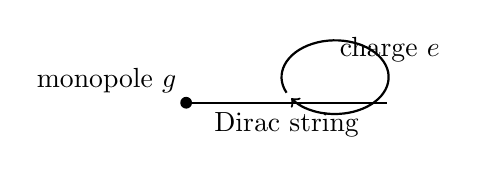
\begin{tikzpicture}[scale=0.85]
      \fill (0,0) circle (2.5pt);
      \node[above left] at (0,0) {monopole \(g\)};
      \draw[thick] (0,0) -- (3.0,0);
      \node[below] at (1.5,0) {Dirac string};
      \draw[->,thick] (1.5,0.15) arc[start angle=205,end angle=-145,
        x radius=0.8,y radius=0.55];
      \node[right] at (2.15,0.8) {charge \(e\)};
    \end{tikzpicture}
    \end{adjustbox}
    \par\smallskip\footnotesize (b) Das Phasenexperiment um die Saite.
  \end{minipage}
  \caption{Die elektrische und die magnetische Ladung sind durch die Dirac-Bedingung umgekehrt proportional verknüpft.}
  \lectureframe{01:13:20}
  \label{fig:l04-dirac-board}
\end{figure}

Ist \(e\) klein, ist die gewöhnliche Störungstheorie in elektrischen Variablen zweckmäßig. Feynman-Diagramme mit zusätzlichen elektrischen Vertizes werden zunehmend unterdrückt. Aus \eqref{eq:l04-dirac-quantization} folgt jedoch, dass \(g\) dann groß ist, sodass eine Diagrammentwicklung in magnetischen Vertizes nicht zweckmäßig ist. Für die üblichen dimensionslosen Kopplungen gilt
\begin{equation}
  \alpha_e=\frac{e^2}{4\pi},
  \qquad
  \alpha_m=\frac{g^2}{4\pi},
  \qquad
  \alpha_e\alpha_m=\frac{n^2}{4}.
  \label{eq:l04-dual-couplings}
\end{equation}
Eine schwache elektrische Kopplung bedeutet eine starke magnetische Kopplung und umgekehrt.

Auch das stark gekoppelte Monopol erscheint in der elektrischen Beschreibung kompliziert. Seine Feldenergie ist groß; es ist von einer intensiven Wolke aus Eichfeldfluktuationen und virtuellen magnetisch geladenen Paaren umgeben. Es verhält sich wie ein schweres, ausgedehntes Objekt und eignet sich schlecht als Ausgangspunkt für eine elektrische Störungsreihe. Das beweist nicht, dass es weniger fundamental ist. Es besagt, dass es in diesem Regime die falsche elementare Variable ist.

Erhöhen wir nun \(e\) kontinuierlich. Die Quantisierungsbedingung zwingt \(g\), abzunehmen. In der Nähe des selbstdualen Bereichs ist keine der beiden Beschreibungen besonders schwach gekoppelt. Jenseits davon können die magnetischen Variablen zu den einfacheren, leichteren werden, während die elektrischen Objekte stark umgeben werden. Welche Ladung als elementar gelten sollte, hat sich geändert, ohne dass sich der physikalische Inhalt der Theorie verändert hätte.

\subsection{Die Frage von Wigner}

Diese Mehrdeutigkeit trat einmal in einer Diskussion darüber auf, ob das Higgs-Boson fundamental oder zusammengesetzt sei. Eugene Wigner fragte wiederholt, was „zusammengesetzt“ bedeute. Als mögliches Unterscheidungsmerkmal wurde der Zerfall vorgeschlagen: Vielleicht könne ein fundamentales Objekt nicht zerfallen, ein zusammengesetztes dagegen schon. Doch ein Wasserstoffatom im Grundzustand kann nicht zerfallen und ist offensichtlich zusammengesetzt; das Proton mag stabil sein, während das Neutron zerfällt, doch dadurch wird im beabsichtigten Sinn nicht das eine elementar und das andere zusammengesetzt. Jede einfache Definition führte zu einem weiteren Gegenbeispiel.

Gerardus ’t Hooft beendete die Diskussion mit einem pragmatischen Kriterium: Ein Objekt ist fundamental, wenn es zweckmäßig ist, es als fundamental zu betrachten. Das ist kein Ausweichen. Es erkennt an, dass „elementar“ die Variablen bezeichnet, in denen die Dynamik einfach ist, und dass diese Einfachheit von Kopplung und Umgebung abhängen kann.

\section{Auf dem Weg zur M-Theorie}

Die Stringtheorie verwirklicht diesen Wechsel der Rollen besonders deutlich. In einem Parameterregime sind Strings leicht und störungstheoretisch behandelbar, während D-Branen als schwere solitonische zusammengesetzte Objekte erscheinen, die aus String-Freiheitsgraden aufgebaut sind. Ändern sich die Parameter, können D-Branen zu den leichteren elementaren Objekten werden, und Konfigurationen, die im ersten Regime als Strings beschrieben wurden, lassen sich nun in diesen Begriffen neu deuten. Was fundamental erschien, kann zusammengesetzt werden; was zusammengesetzt erschien, kann fundamental werden.

Das ältere reduktionistische Bild legt einen geradlinigen Abstieg von großen Dingen zu kleineren Bestandteilen und schließlich zu einer einzigen untersten Ebene nahe. Dualität deutet auf etwas weniger Lineares hin: Beschreibungen können sich bei veränderlichen Kopplungen ineinander überführen lassen, ohne dass ein einziger Variablensatz überall Vorrang hat. Aus dieser Perspektive wenden wir uns als Nächstes der M-Theorie zu.

Die Frage, warum die kritischen Dimensionen für den bosonischen String sechsundzwanzig und für den Superstring zehn betragen, bleibt hier offen. Statt vor dem Weitergehen jedes technische Problem zu klären, wechseln wir nun die Perspektive und fragen, wie die M-Theorie in einem geeigneten Limes die Stringtheorie hervorbringen kann.